\chapter{}
\label{lecture15}
\section{Колебания мембраны.}
\label{lecture15section1}
\begin{_def}
	\textbf{Мембрана} --- двумерный аналог струны. Это тонкая плёна не сопротивляется изгибу, а сопротивляется растяжению.
\end{_def}
Мы считаем, что эта плёнка натянута на некоторую плоскую кривую, ограничивающую область $G$. Выберем систему координат так, чтобы область $G$ лежала в плоскости $x0y$. Обозначим через $u(x,y,t)$ смещение точки $x,y$ в момент $t$ и будем предполагать,
\begin{enumerate1}
	\item что смещения ортогональны к плоскости $x0y$,
	\item что колебания (смещения) малы.
\end{enumerate1}




\tikzset{every picture/.style={line width=0.75pt}} %set default line width to 0.75pt        

\begin{tikzpicture}[x=0.75pt,y=0.75pt,yscale=-1,xscale=1]
	%uncomment if require: \path (0,269); %set diagram left start at 0, and has height of 269
	
	%Straight Lines [id:da1467503181774934] 
	\draw    (122.98,164.3) -- (305.78,164.3) ;
	\draw [shift={(307.78,164.3)}, rotate = 180] [color={rgb, 255:red, 0; green, 0; blue, 0 }  ][line width=0.75]    (10.93,-3.29) .. controls (6.95,-1.4) and (3.31,-0.3) .. (0,0) .. controls (3.31,0.3) and (6.95,1.4) .. (10.93,3.29)   ;
	%Straight Lines [id:da8912290272812766] 
	\draw    (122.98,164.3) -- (34.23,249.47) ;
	\draw [shift={(32.78,250.85)}, rotate = 316.18] [color={rgb, 255:red, 0; green, 0; blue, 0 }  ][line width=0.75]    (10.93,-3.29) .. controls (6.95,-1.4) and (3.31,-0.3) .. (0,0) .. controls (3.31,0.3) and (6.95,1.4) .. (10.93,3.29)   ;
	%Straight Lines [id:da6656158631721258] 
	\draw    (122.98,164.3) -- (122.98,10.85) ;
	\draw [shift={(122.98,8.85)}, rotate = 450] [color={rgb, 255:red, 0; green, 0; blue, 0 }  ][line width=0.75]    (10.93,-3.29) .. controls (6.95,-1.4) and (3.31,-0.3) .. (0,0) .. controls (3.31,0.3) and (6.95,1.4) .. (10.93,3.29)   ;
	%Shape: Polygon Curved [id:ds7634331840148227] 
	\draw   (166.78,186.87) .. controls (161.78,172.87) and (200.78,171.87) .. (215.78,182.87) .. controls (230.78,193.87) and (244.57,207.74) .. (224.78,225.87) .. controls (205,244) and (148.78,234.87) .. (156.78,221.87) .. controls (164.78,208.87) and (171.78,200.87) .. (166.78,186.87) -- cycle ;
	
	% Text Node
	\draw (19,242.4) node [anchor=north west][inner sep=0.75pt]    {$x$};
	% Text Node
	\draw (308.78,161.7) node [anchor=north west][inner sep=0.75pt]    {$y$};
	% Text Node
	\draw (128,2.39) node [anchor=north west][inner sep=0.75pt]    {$u( x,y,t)$};
	% Text Node
	\draw (124.98,167.7) node [anchor=north west][inner sep=0.75pt]    {$0$};
	% Text Node
	\draw (191,196.4) node [anchor=north west][inner sep=0.75pt]    {$G$};
	
	
\end{tikzpicture}

Вывод уравнения колебаний мембраны мы проведём с помощью принципа Гамильтона так же, как выводили уравнение колебаний струны. Составим интеграл действия
\begin{equation*}
	\hfill\J[u]=\int\limits_{t_0}^{t_1}(T-V)\,dt\hfill
\end{equation*}
и затем из условия $\delta\J=0$ получим уравнение колебаний и граничные условия. Пусть $\rho(x,y,t)$ --- плотность мембраны. Тогда очевидно, что кинетическая энергия мембраны 
\begin{equation}\label{l15:eq:1}
	\hfill T=\frac{1}{2}\cdot\iint\limits_{G}\rho\cdot u_t^2\,dxdy,\hfill
\end{equation} 
потенциальная энергия
\begin{equation}\label{l15:eq:2}
	\hfill V=V_1+V_2,\hfill
\end{equation} 
где $V_1$ --- потенциальная энергия мембраны за счёт растяжения, а $V_2$ --- за счёт работы внешних сил.

Пусть $\Delta G$ --- элементарный участок мембраны. Его потенциальная энергия за счёт растяжения мембраны пропорциональна увеличению площади, а коэффициентом пропорциональности $\mu$ является модуль упругости
\begin{equation*}
	\hfill\Delta V_1=\mu\cdot\left(\sqrt{1+u_x^2+u_y^2}\cdot\Delta G-\Delta G\right)\approx\mu\cdot\frac{u_x^2+u_y^2}{2}\cdot\Delta G.\hfill
\end{equation*}
Откуда
\begin{equation}\label{l15:eq:3}
	\hfill V_1=\iint\limits_{G}\frac{\mu}{2}\cdot(u_x^2+u_y^2)\,dG.\hfill
\end{equation}
При выводе~\eqref{l15:eq:3} аналогично случаю малых колебаний струны мы использовали малость $|u_x|$ и $|u_y|$ для приближённого вычисления $\sqrt{1+u_x^2+u_y^2}$.

Пусть на мембрану действует распределённая сила $\mc{F}$, направленная перпендикулярно к плоскости $x0y$ и $f(x,y,t)$ --- плотность этой силы на единицу площади. Тогда сила $\Delta\mc{F}$, действующая на участок $\Delta G$,есть $\Delta\mc{F}=f(x,y,t)\cdot\Delta G$, её потенциал $\Delta U=-f(x,y,t)\cdot u(x,y,t)\cdot\Delta G$, а элементарная потенциальная энергия за счёт действия силы $\Delta \mc{F}$ есть $\Delta V_{2}=-f\cdot u\cdot\Delta G$. Поэтому 
\begin{equation}\label{l15:eq:4}
	\hfill V_{2}=-\iint\limits_{G}f\cdot u\,dG.\hfill
\end{equation}
Если бы на границу мембраны $\Gamma=\partial G$ действовала распределённая сила с линейной плотностью $g(x,y,t)$, то к потенциальной энергии $V$ надо было добавить
\begin{equation}\label{l15:eq:5}
	\hfill V_{\Gamma}=-\int\limits_{\Gamma}g(x,y,t)\cdot u(x,y,t)\,d\Gamma.\hfill
\end{equation}  
Однако мы этого делать не будем, считая пока $g\equiv0$.

В формулах для кинетической и потенциальной энергии мембраны нет слагаемых, отвечающих за изменение энергии за счёт сосредоточенных источников. Как учесть эти источники, если они есть? Пусть, например, в точке $\overline{x}$, $\overline{y}$ к мембране прикреплена точечная масса $\overline{m}$. <<Размажем>> массу $\overline{m}$ по $\alpha$ --- окрестности ($|\alpha|\ll1$) точки $\overline{x}$, $\overline{y}$ и таким образом к плотности мембраны $\rho(x,y,t)$ в формуле кинетической энергии надо будет добавить плотность $\rho_{\alpha}$ за счёт размазывания и решать задачу с плотностью мембраны $\rho+\rho_{\alpha}$, а потом переходить к пределу при $\alpha\to0$. <<Размазывание>> можно осуществить, например, так. Пусть $h_{\alpha}(x,y)$ --- любая последовательность непрерывных в области $G$ функций, обладающих следующими свойствами 
\begin{equation*}
	\hfill\left\{\begin{array}{ccc}
		h_{\alpha}\equiv0&\text{при}&(x-\overline{x})^2+(y-\overline{y})^2\geqslant\alpha^2,\\
		h_{\alpha}>0&\text{при}&(x-\overline{x})^2+(y-\overline{y})^2<\alpha^2,
	\end{array}\right. \qquad\text{и}\quad\iint\limits_{G}h_{\alpha}(x,y)\,d\alpha=1,\quad\forall\alpha>0.\hfill
\end{equation*} 
Тогда положим 
\begin{equation*}
	\hfill\rho_{\alpha}(x,y)=\overline{m}\cdot h_{\alpha}(x,y).\hfill
\end{equation*} 
Очевидно, масса, добавленная за счёт размазывания
\begin{equation*}
	\hfill\iint\limits_{G}\overline{m}\cdot h_{\alpha}(x,y)\,dG=\overline{m}\hfill
\end{equation*}
и $\rho_{\alpha}(x,y)=0$, $|x-\overline{x}|^2+|y-\overline{y}|^2\geqslant\alpha^2$.

Аналогично учитывается действие сосредоточенной силы. Пусть в точке $\overline{x}$, $\overline{y}$ на мембрану действует перпендикулярная к плоскости $x0y$ сосредоточенная сила $\overline{\mc{F}}(t)$. <<Размажем>> её по $\alpha$-окрестности точки $\overline{x}$, $\overline{y}$ так же, как мы размазывали массу $\overline{m}$, введя плотность полученной распределённой силы $\overline{\mc{F}}_{\alpha}(x,y,t)$ по формуле
\begin{equation*}
	\hfill \overline{f}_{\alpha}(x,y,t)=\overline{\mc{F}}\cdot h_{\alpha}(x,y),\hfill
\end{equation*}
где $h_{\alpha}(x,y)$ --- то же, что и выше. Тогда в выражении $V_{2}$ мы должны будем вместо $f(x,y,t)$ написать $f(x,y,t)+\overline{f}_{\alpha}(x,y,t)$.

Далее считаем, что сосредоточенных источников изменения потенциальной энергии нет. В силу~\eqref{l15:eq:1}---\eqref{l15:eq:4} интеграл действия запишется в виде
\begin{equation*}
	\hfill\J[u]=\int\limits_{t_0}^{t_1}\!\iint\limits_{G}\left[\frac{1}{2}\cdot\rho\cdot u_t^2-\frac{1}{2}\cdot\mu\cdot(u_x^2+u_y^2)+f\cdot u\right]\,dGdt.\hfill
\end{equation*}
Обозначим подынтегральное выражение через $F(x,y,t,u,u_x,u_y,u_t)$ и из равенства нулю первой вариации: $\delta\J=0$ получаем уравнение Остроградского
\begin{equation*}
	\hfill F_u-\der{}{x}F_{u_x}-\der{}{y}F_{u_y}-\der{}{t}F_{u_t}=0,\hfill
\end{equation*}
которое после подстановки $F$ и даёт уравнение колебаний мембраны
\begin{equation}\label{l15:eq:6}
	\hfill f+\pder{}{x}\big(\mu\cdot u_x\big)+\pder{}{y}\big(\mu\cdot u_y\big)-\pder{}{t}\big(\rho\cdot u_t\big)=0\footnotemark{}.\hfill
\end{equation}\footnotetext{Здесь не важно $\pder{}{x}$ или $\der{}{x}$, $\pder{}{y}$ или $\der{}{y}$ и так далее.}%
Далее рассматриваем однородную мембрану: $\rho$ и $\mu$ --- константы. Полагая $a^2\eqdef\mu\!\bigm/\!\rho$ и поделив~\eqref{l15:eq:6} на $\rho$ запишем полученное уравнение в виде
\begin{equation}\label{l15:eq:7}
	\hfill u_{tt}=a^2\cdot\Delta u+\frac{f}{\rho},\hfill
\end{equation}
где $\displaystyle\Delta u=\pdder{u}{x}+\pdder{u}{y}$.

Для нахождения единственного решения мы должны задать начальные и граничные условия. Начальные
\begin{equation}\label{l15:eq:8}
	\hfill u(x,y,0)=\phi(x,y),\quad u_t(x,y,0)=\psi(x,y).\hfill
\end{equation}
Что касается граничных условий, то в случае закреплённого края $\left(u\Big|_{\partial G}=0\right)$ и в случае задания закона движения края $\left(u\Big|_{\partial G}=\nu(x,y,t)\right)$ эти условия просто задаются, а в остальных случаях (см. ниже) выводятся как естественные граничные условия аналогично выводу для колебаний струны. Эти условия даны ниже:
\begin{enumerateD}
	\item cвободная граница: $\displaystyle \left.\pder{u}{n}\right|_{\partial G}=0$,
	\item наличие на границе распределённой силы с линейной плотностью $g(x,y,t)$: $\displaystyle \left.\pder{u}{n}\right|_{\partial G}=\frac{g}{\mu}$,
	\item упругое закрепление границы: $\displaystyle\left.\pder{u}{n}+\sigma\cdot u\right|_{\partial G}=0$, $\sigma>0$. 
\end{enumerateD}
Отметим, что аналогично тому, что на концах струны могут быть различные граничные условия, так и на разных участках границы $\partial G$ возможно задание различных условий. Например, если $\Gamma=\partial G$, то на части $\Gamma_1$ кривой $\Gamma$ может быть закрепление, а другая часть $\Gamma_2$ может быть свободной.
\vspace{0.2cm}


\tikzset{every picture/.style={line width=0.75pt}} %set default line width to 0.75pt        

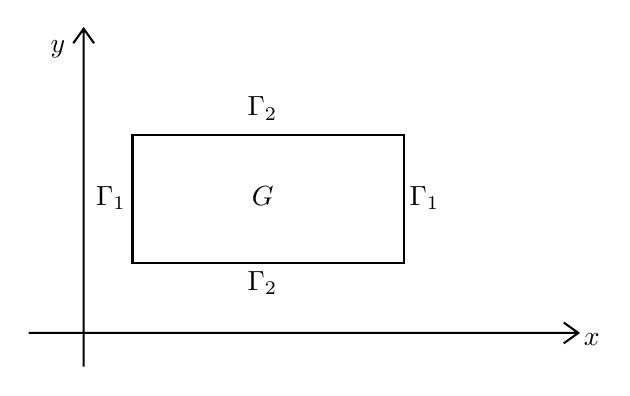
\begin{tikzpicture}[x=0.75pt,y=0.75pt,yscale=-1,xscale=1]
	%uncomment if require: \path (0,222); %set diagram left start at 0, and has height of 222
	
	%Shape: Axis 2D [id:dp3319617018609984] 
	\draw  (33,173.57) -- (297.78,173.57)(59.48,27) -- (59.48,189.85) (290.78,168.57) -- (297.78,173.57) -- (290.78,178.57) (54.48,34) -- (59.48,27) -- (64.48,34)  ;
	%Shape: Rectangle [id:dp5822068251009356] 
	\draw   (83,78) -- (213.78,78) -- (213.78,139.85) -- (83,139.85) -- cycle ;
	
	% Text Node
	\draw (299,172.4) node [anchor=north west][inner sep=0.75pt]    {$x$};
	% Text Node
	\draw (42,31.4) node [anchor=north west][inner sep=0.75pt]    {$y$};
	% Text Node
	\draw (64,101.4) node [anchor=north west][inner sep=0.75pt]    {$\Gamma _{1}$};
	% Text Node
	\draw (215,101.4) node [anchor=north west][inner sep=0.75pt]    {$\Gamma _{1}$};
	% Text Node
	\draw (137,142.4) node [anchor=north west][inner sep=0.75pt]    {$\Gamma _{2}$};
	% Text Node
	\draw (137,58.4) node [anchor=north west][inner sep=0.75pt]    {$\Gamma _{2}$};
	% Text Node
	\draw (139,101.4) node [anchor=north west][inner sep=0.75pt]    {$G$};
	
	
\end{tikzpicture}

Теорема о единственности решения уравнения~\eqref{l15:eq:6} доказывается с помощью интеграла энергии аналогично случаю струны.

Рассмотрим задачу о свободных колебаниях однородной мембраны. То есть решаем уравнение~\eqref{l15:eq:7} с $f(x,y,t)\equiv0$, начальными условиями~\eqref{l15:eq:8} и однородными граничными условиями закрепления
\begin{equation}\label{l15:eq:9}
	\hfill u\Big|_{\partial G}=0\hfill
\end{equation}
или со свободной границей
\begin{equation}\label{l15:eq:10}
	\hfill \left.\pder{u}{n}\right|_{\partial G}=0.\hfill
\end{equation}

Решение ищем методом Фурье. Сначала пытаемся найти частное решение только для уравнения~\eqref{l15:eq:7} и граничных условий~\eqref{l15:eq:9} или~\eqref{l15:eq:10}. Пусть для краткости $P=(x,y)$. Имеем
\begin{equation*}
	\hfill u_{\text{ч}}(P,t)=v(P)\cdot T(t).\hfill
\end{equation*}
Подставив в~\eqref{l15:eq:7} и поделив потом на произведение $v\cdot T\cdot a^2$ получим аналогично задаче о колебаниях струны 
\begin{equation*}
	\hfill \frac{T''}{a^2\cdot T}=\frac{\Delta v}{v}=-\lambda,\hfill
\end{equation*} 
откуда 
\begin{equation}\label{l15:eq:11}
	\hfill T''+\lambda\cdot a^2\cdot T=0,\hfill
\end{equation}
\begin{equation}\label{l15:eq:12}
	\hfill -\Delta v=\lambda\cdot v.\hfill
\end{equation}
Из~\eqref{l15:eq:9} и~\eqref{l15:eq:10} получаем, что 
\begin{equation}\label{l15:eq:13}
	\hfill v\Big|_{\partial G}=0\hfill
\end{equation}
или 
\begin{equation}\label{l15:eq:14}
	\hfill \left.\pder{v}{n}\right|_{\partial G}=0.\hfill
\end{equation}

В курсе вариационного исчисления мы говорили о том, что у оператора $(-\Delta)$ существует бесконечная последовательность собственных значений $\lambda_n$ $\lambda_1<\lambda_2\leqslant\lambda_3\leqslant\ldots$, где каждое собственно езначение повторяется число раз, равное размерности собственного подпространства. Пусть $v_n(P)$ --- соответствующие ортонормированные собственные функции. Из~\eqref{l15:eq:11} мы получим
\begin{equation*}
	\hfill \begin{array}{rclll}
		T_n(t)&=&A_n\cdot\cos\left(\omega_n\cdot t\right)+B_n\cdot\sin\left(\omega_n\cdot t\right)&\text{при}&\lambda_n>0,\ n=1,2,\ldots,\\
		T_1(t)&=&A_1+B_1\cdot t&\text{при}&\lambda_1=0,
	\end{array}\hfill
\end{equation*}
где $\omega_n=a\cdot\sqrt{\lambda_n}$\footnote{Напоминаю, что при свободной границе, то есть при условии~\eqref{l15:eq:14} --- наименьшее собственное значение $\lambda_1=0$, ему отвечает нормированная собственная функция $v_1=1\!\!\Bigm/\!\!\!\sqrt{S(G)}$, где $S(G)$ --- площадь области $G$.}. 

Таким образом
\begin{equation*}
	\hfill u_{\text{ч}}=u_{n}(P,t)=v_{n}(P)\cdot T_{n}(t).\hfill
\end{equation*}
Положим 
\begin{equation}\label{l15:eq:15}
	\hfill u\eqdef\sum\limits_{n=1}^{\infty}v_n(P)\cdot T_n(t).\hfill
\end{equation}
Если ряд~\eqref{l15:eq:15} сходится равномерно при выбранных $A_n$, $B_n$ и допускает двукратное почленное дифференцирование по $x$, $y$, $t$, то~\eqref{l15:eq:15} есть решение~\eqref{l15:eq:7} (при $f=0$) и функция $u$ удовлетворяем граничному условию (\eqref{l15:eq:13} или~\eqref{l15:eq:14}). Далее пытаемся подобрать числа $A_n$ и $B_n$ в выражении $T_n(t)$ так, чтобы выполнялись начальные условия~\eqref{l15:eq:8}. Имеем
\begin{equation}\label{l15:eq:16}
	u(P,0)=\sum\limits_{n=1}^{\infty}T_n(0)\cdot v_n(P)=\sum\limits_{n=1}^{\infty}A_n\cdot v_n(P)=\phi(P),
\end{equation}
\begin{equation}\label{l15:eq:17}
	u_t(P,0)=\sum\limits_{n=1}^{\infty}T'_n(0)\cdot v_n(P)=\sum\limits_{n=1}^{\infty}\omega_n\cdot B_n\cdot v_n(P)=\psi(P).
\end{equation}
По теореме Стеклова для оператора Лапласа разложения~\eqref{l15:eq:16} и~\eqref{l15:eq:17} возможны при соответствующих свойствах $\phi(P)$ и $\psi(P)$ и
\begin{multline*}
	A_n=\big(\phi(P),v_n(P)\big)=\iint\limits_{G}\phi(P)\cdot\overline{v}_n(P)\,dG;\\\omega_n\cdot B_n=\big(\psi(P),v_n(P)\big)=\iint\limits_{G}\psi(P)\cdot\overline{v}_n(P)\,dG\quad
	\Rightarrow\quad B_n=\big(\psi(P),v_n(P)\big)\cdot\omega_n^{-1}.
\end{multline*}

Таким образом мы можем решить поставленную задачу, если знать собственные значения и собственные функции оператора Лапласа --- $\lambda_n$ и $v_n$. Увы, их аналитическое нахождение возможно лишь для области $G$ специального вида, а в общем случае они могут быть найдены только численно.

Заметим, что в рассмотренных позже случаях, когда нахождение $\lambda_n$ и $v_n$ возможно, индекс $n$ будет векторным (мультииндексом) скажем $\bm{n}=(k,m)$ или $\bm{n}=(k,m,i)$ однако все проведённые выше рассуждения сохраняются и в этом случае.
\section{Вынужденные колебания однородной мембраны.}
\label{lecture15section2}
Мы будем изучать вынужденные колебания мембраны при наличии внешней распределённой силы с плотностью $f(x,y,t)$ на единицу площади. Тогда в силу~\eqref{l15:eq:7} в уравнение колебаний войдёт плотность $\widetilde{f}\eqdef f\!\bigm/\!\rho$ на единицу массы и~\eqref{l15:eq:7} примет вид
\begin{equation}\label{l15:eq:18}
	\hfill\pdder{u}{t}=a^2\cdot\Delta u+\widetilde{f}.\hfill
\end{equation}
Мы будем решать~\eqref{l15:eq:18} при тех же начальных и граничных условиях что и в задаче о свободных колебаниях:
\begin{equation}\label{l15:eq:19}
	\hfill u(P,0)=\phi(P),\quad u_t(P,0)=\psi(P),\hfill
\end{equation} 
\begin{equation}\label{l15:eq:20}
	\hfill u\Big|_{\partial G}=0\hfill
\end{equation} 
или
\begin{equation}\label{l15:eq:21}
	\hfill \left. \pdder{u}{n}\right|_{\partial G}=0.\hfill
\end{equation} 
Как и в задаче о колебаниях струны, надо найти решение уравнения~\eqref{l15:eq:18} с граничными условиями~\eqref{l15:eq:20} или~\eqref{l15:eq:21}, а потом добавить к нему решение~\eqref{l15:eq:18} с $\widetilde{f}=0$ и подходящими начальными условиями.

Рассмотрим сначала случай стационарной силы: $\widetilde{f}=\widetilde{f}(P)$. Разложим функцию $\widetilde{f}(P)$ по собственным функциям $v_n(P)$ оператора Лапласа и будем искать стационарное решение~\eqref{l15:eq:18}, то есть решение уравнения
\begin{equation}\label{l15:eq:22}
	\hfill-a^2\cdot\Delta u=\widetilde{f}(P),\hfill
\end{equation}
в виде ряда $\displaystyle u=\sum\limits_{n=1}^{\infty}C_n\cdot v_n$ с неизвестными коэффициентами $C_n$. Подставляя в~\eqref{l15:eq:22} разложение для $u$ и $\widetilde{f}$ и учитывая, что $-\Delta v_n=\lambda_n\cdot v_n$ получим
\begin{equation}\label{l15:eq:23}
	\hfill\sum\limits_{n=1}^{\infty}a^2\cdot C_n\cdot v_n\cdot\lambda_n=\sum\limits_{n=1}^{\infty}\widetilde{f}_n\cdot v_n,\hfill
\end{equation}
где $\widetilde{f}_n=\big(\widetilde{f},v_n\big)$. Из~\eqref{l15:eq:23} получаем
\begin{equation*}
	\hfill a^2\cdot C_n\cdot\lambda_n=\widetilde{f}_n,\hfill
\end{equation*}
откуда при $\lambda_n\neq0\quad$$\displaystyle C_n=\frac{\widetilde{f}}{a^2\cdot\lambda_n}$. Если мы работали с условием~\eqref{l15:eq:20}, то $\lambda_n>0$, $n=1,2,\ldots$ и задача нахождения решения $u$ выполнена. Если было условие~\eqref{l15:eq:21}, то $\lambda_1=0$ и решение существует лишь при $\widetilde{f}_1=0$, то есть когда 
\begin{equation*}
	\hfill\iint\limits_{G} \widetilde{f}(P)\cdot\frac{1}{\sqrt{S(G)}}\,dG=0\hfill
\end{equation*}
--- результирующая сила, действующая на мембрану, равна нулю. Ясно, что при не выполнении этого условия мембрана со свободной границей двигалась бы как целое и стационарного решения не существовало бы. Ясно, что при $\lambda_1=0$ (и $\widetilde{f}_1=0$) величина $C_1$ --- произвольна.  

Рассмотрим теперь вынужденные колебания однородной мембраны под действием не стационарной силы. Решение~\eqref{l15:eq:18} ищем в виде
\begin{equation*}
	\hfill u=\widehat{u}+w,\hfill
\end{equation*}
где $\widehat{u}$ --- решение однородного уравнения
\begin{equation*}
	\hfill \widehat{u}_{tt}=a^2\cdot\Delta\widehat{u}\hfill
\end{equation*}
с граничными условиями задачи и начальными условиями 
\begin{equation}\label{l15:eq:24}
	\hfill\widehat{u}(P,u)=\phi(P)-w(P,0),\quad \widehat{u}_t(P,0)=\psi(P)-w_t(P,0),\hfill
\end{equation}
а $w(P,t)$ --- новая неизвестная функция. Подставив $u$ в уравнение~\eqref{l15:eq:18} и в граничные условия~\eqref{l15:eq:20},~\eqref{l15:eq:21} видим, что функция $w(P,t)$ должна удовлетворять~\eqref{l15:eq:18} и~\eqref{l15:eq:20} (или~\eqref{l15:eq:21}), а о начальных условиях для $w(P,t)$ в силу~\eqref{l15:eq:24} можно не беспокоиться. Обычно выбирают или
\begin{equation*}
	\hfill w(P,0)=w_t(P,0)=0\hfill
\end{equation*} 
и тогда для $\widehat{u}$ будут исходные начальные условия~\eqref{l15:eq:8} или берут 
\begin{equation*}
	\hfill w(P,0)=\phi,\quad w_t(P,0)=\psi\hfill
\end{equation*} 
и тогда функция $\widehat{u}\equiv0$, а $w(P,t)$ и есть решение задачи~\eqref{l15:eq:18},~\eqref{l15:eq:19} и~\eqref{l15:eq:20} (или~\eqref{l15:eq:21}). Ищем $w(P,t)$ в виде ряда по собственным функциям $v_n(P)$ оператора Лапласа:
\begin{equation}\label{l15:eq:25}
	\hfill w(P,t)=\sum\limits_{n=1}^{\infty}b_n(t)\cdot v_n(P).\hfill
\end{equation}
Разложение~\eqref{l15:eq:25} --- это результат применения теоремы Стеклова к функции $w(P,t)$ при фиксированном $t$. Разложим аналогично функцию $\widetilde{f}(P,t)$:
\begin{equation}\label{l15:eq:26}
	\hfill\widetilde{f}(P,t)=\sum\limits_{n=1}^{\infty}\widetilde{f}_n(t)\cdot v_n(P)\hfill
\end{equation}
и подставим~\eqref{l15:eq:25} и~\eqref{l15:eq:26} в~\eqref{l15:eq:18}. Тогда, учитывая, что $\Delta v_n=-\lambda_n\cdot v_n$ получим 
\begin{equation*}
	\hfill\sum\limits_{n=1}^{\infty}b_n''\cdot v_n=-a^2\cdot\sum\limits_{n=1}^{\infty}\lambda_n\cdot v_n\cdot b_n+\sum\limits_{n=1}^{\infty}\widetilde{f}_n(t)\cdot v_n\hfill
\end{equation*}
откуда следует, что 
\begin{equation}\label{l15:eq:27}
	\hfill b_n''+\omega_n^2\cdot b_n=\widetilde{f}_n(t),\quad n=1,2,\ldots\,.\hfill
\end{equation}
Из~\eqref{l15:eq:25} получаем начальные условия для решений $b_n(t)$ уравнения~\eqref{l15:eq:27}
\begin{equation*}
	\hfill\begin{array}{rcccl}
		b_n(0)&=&\big(w(P,0),v_n\big)&=&\displaystyle\iint\limits_{G}w(P,0)\cdot v_n(P)dG,\\
		b'_n(0)&=&\big(w_t(P,0),v_n\big)&=&\displaystyle\iint\limits_{G}w_t(P,0)\cdot v_n(P)dG.
	\end{array}\hfill
\end{equation*}
Если взять $w(P,0)=w'(P,0)=0$, то $b_n(0)=b_n'(0)=0$ и аналогияно случаю вынужденных колебаний струны (лекция~13) мы получим 
\begin{equation*}
	\hfill b_n(t)=\frac{1}{\omega_n}\cdot\int\limits_0^t\sin\left(\omega_n\cdot(t-\tau)\right)\cdot\widetilde{f}_n(\tau)\,d\tau=\frac{1}{\omega_n}\cdot\int\limits_0^t\iint\limits_{G}\sin\left(\omega_n\cdot(t-\tau)\right)\cdot\widetilde{f}(P,\tau)\cdot v_n(P)\,dGd\tau.\hfill
\end{equation*}
Таким образом функция $w(P,t)$ найдена, а способ отыскания $\widehat{u}(P,t)$ описан ранее.